\documentclass{standalone}
\usepackage{tikz}
\usetikzlibrary{patterns, positioning}
\usepackage[sfdefault]{ClearSans} %% option 'sfdefault' activates Clear Sans as the default text font
\usepackage[T1]{fontenc}

\begin{document}
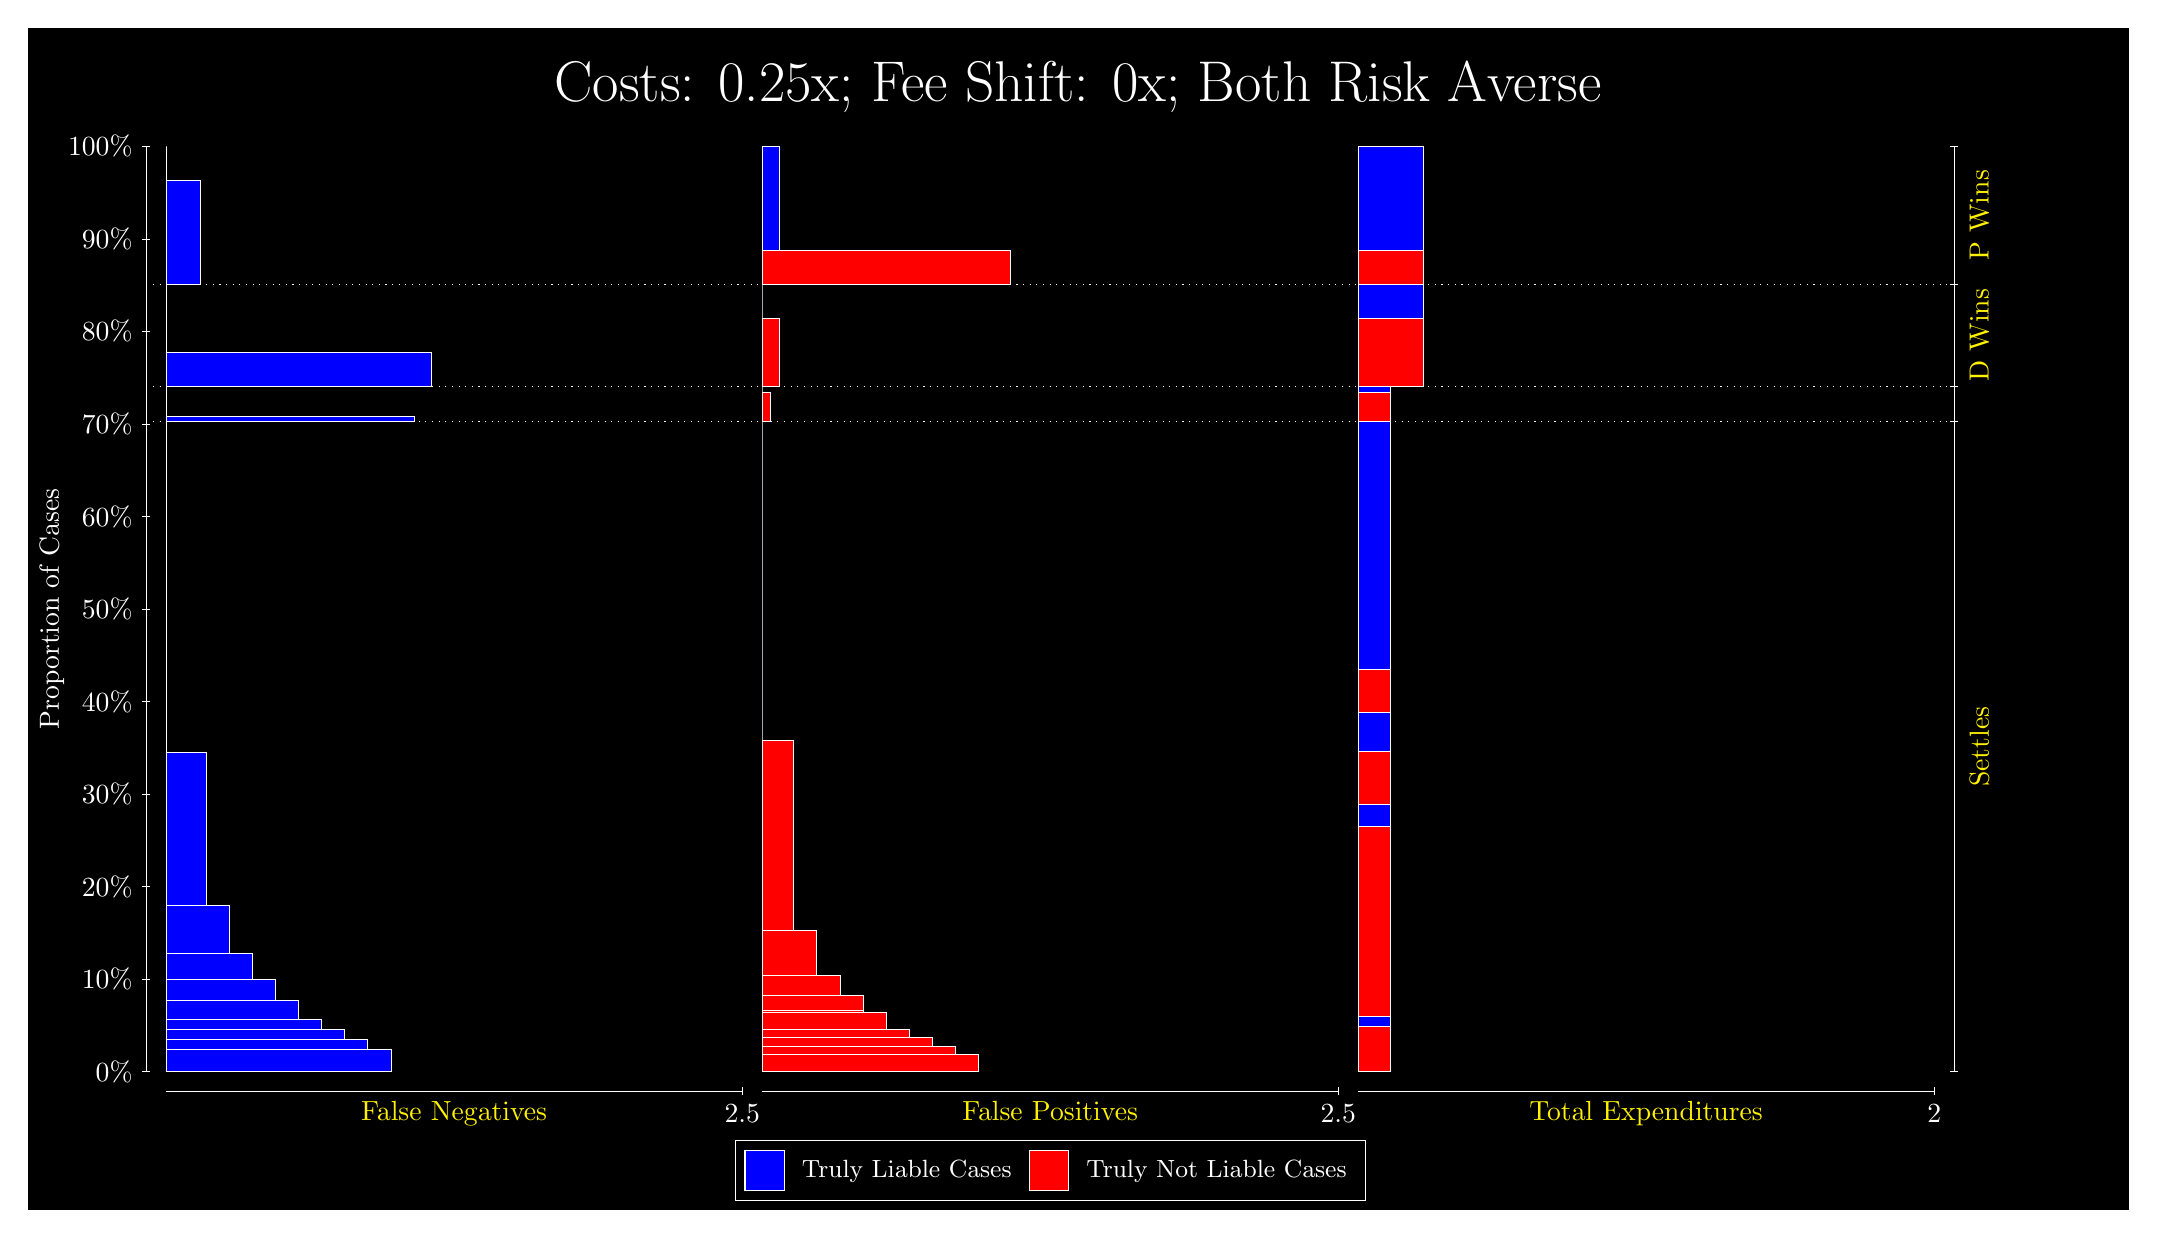
\begin{tikzpicture}
\draw[fill=black] (0,0) rectangle (26.667,15);
\draw[text=white] (0,13.5) rectangle (26.667,15) node[midway] {\huge Costs: 0.25x; Fee Shift: 0x; Both Risk Averse};
\draw[white, very thin] (1.5,1.75) -- (1.5,13.5);
\node[rotate=90, text=white, anchor=center] at (0.3, 7.625) {Proportion of Cases};
\draw[white, very thin] (1.45,1.75) -- (1.55,1.75);
\node[text=white, anchor=east] at (1.45, 1.75) {0\%};
\draw[white, very thin] (1.45,2.925) -- (1.55,2.925);
\node[text=white, anchor=east] at (1.45, 2.925) {10\%};
\draw[white, very thin] (1.45,4.1) -- (1.55,4.1);
\node[text=white, anchor=east] at (1.45, 4.1) {20\%};
\draw[white, very thin] (1.45,5.275) -- (1.55,5.275);
\node[text=white, anchor=east] at (1.45, 5.275) {30\%};
\draw[white, very thin] (1.45,6.45) -- (1.55,6.45);
\node[text=white, anchor=east] at (1.45, 6.45) {40\%};
\draw[white, very thin] (1.45,7.625) -- (1.55,7.625);
\node[text=white, anchor=east] at (1.45, 7.625) {50\%};
\draw[white, very thin] (1.45,8.8) -- (1.55,8.8);
\node[text=white, anchor=east] at (1.45, 8.8) {60\%};
\draw[white, very thin] (1.45,9.975) -- (1.55,9.975);
\node[text=white, anchor=east] at (1.45, 9.975) {70\%};
\draw[white, very thin] (1.45,11.15) -- (1.55,11.15);
\node[text=white, anchor=east] at (1.45, 11.15) {80\%};
\draw[white, very thin] (1.45,12.325) -- (1.55,12.325);
\node[text=white, anchor=east] at (1.45, 12.325) {90\%};
\draw[white, very thin] (1.45,13.5) -- (1.55,13.5);
\node[text=white, anchor=east] at (1.45, 13.5) {100\%};

\draw[white, very thin] (24.457,1.75) -- (24.457,13.5);
\draw[white, very thin] (24.407,1.75) -- (24.507,1.75);
\node[anchor=west] at (24.407, 1.75) {};
\draw[white, very thin] (24.407,10.002) -- (24.507,10.002);
\node[anchor=west] at (24.407, 10.002) {};
\draw[white, very thin] (24.407,10.455) -- (24.507,10.455);
\node[anchor=west] at (24.407, 10.455) {};
\draw[white, very thin] (24.407,11.747) -- (24.507,11.747);
\node[anchor=west] at (24.407, 11.747) {};
\draw[white, very thin] (24.407,13.5) -- (24.507,13.5);
\node[anchor=west] at (24.407, 13.5) {};

\draw[white, very thin, fill=blue] (1.75,1.75) rectangle (4.6044,2.0369);
\draw[white, very thin, fill=blue] (1.75,2.0369) rectangle (4.3116,2.1636);
\draw[white, very thin, fill=blue] (1.75,2.1636) rectangle (4.0188,2.2872);
\draw[white, very thin, fill=blue] (1.75,2.2872) rectangle (3.7261,2.4106);
\draw[white, very thin, fill=blue] (1.75,2.4106) rectangle (3.4333,2.6561);
\draw[white, very thin, fill=blue] (1.75,2.6561) rectangle (3.1406,2.9217);
\draw[white, very thin, fill=blue] (1.75,2.9217) rectangle (2.8478,3.2529);
\draw[white, very thin, fill=blue] (1.75,3.2529) rectangle (2.5551,3.8639);
\draw[white, very thin, fill=blue] (1.75,3.8639) rectangle (2.2623,5.8012);
\draw[white, very thin, fill=red] (1.75,5.8012) rectangle (1.75,10.002);
\draw[white, very thin, fill=blue] (1.75,10.002) rectangle (4.8971,10.075);
\draw[white, very thin, fill=red] (1.75,10.075) rectangle (1.75,10.455);
\draw[white, very thin, fill=blue] (1.75,10.455) rectangle (5.1167,10.889);
\draw[white, very thin, fill=red] (1.75,10.889) rectangle (1.75,11.747);
\draw[white, very thin, fill=blue] (1.75,11.747) rectangle (2.1891,13.064);
\draw[white, very thin, fill=red] (1.75,13.064) rectangle (1.75,13.5);
\draw[white, very thin, fill=red] (9.3189,1.75) rectangle (12.063,1.9631);
\draw[white, very thin, fill=red] (9.3189,1.9631) rectangle (11.771,2.0701);
\draw[white, very thin, fill=red] (9.3189,2.0701) rectangle (11.478,2.1847);
\draw[white, very thin, fill=red] (9.3189,2.1847) rectangle (11.185,2.2919);
\draw[white, very thin, fill=red] (9.3189,2.2919) rectangle (10.892,2.497);
\draw[white, very thin, fill=red] (9.3189,2.497) rectangle (10.6,2.529);
\draw[white, very thin, fill=red] (9.3189,2.529) rectangle (10.6,2.7206);
\draw[white, very thin, fill=red] (9.3189,2.7206) rectangle (10.307,2.9671);
\draw[white, very thin, fill=red] (9.3189,2.9671) rectangle (10.014,3.5401);
\draw[white, very thin, fill=red] (9.3189,3.5401) rectangle (9.7214,5.9507);
\draw[white, very thin, fill=blue] (9.3189,5.9507) rectangle (9.3189,10.002);
\draw[white, very thin, fill=red] (9.3189,10.002) rectangle (9.4287,10.382);
\draw[white, very thin, fill=blue] (9.3189,10.382) rectangle (9.3189,10.455);
\draw[white, very thin, fill=red] (9.3189,10.455) rectangle (9.5384,11.314);
\draw[white, very thin, fill=blue] (9.3189,11.314) rectangle (9.3189,11.747);
\draw[white, very thin, fill=red] (9.3189,11.747) rectangle (12.466,12.183);
\draw[white, very thin, fill=blue] (9.3189,12.183) rectangle (9.5384,13.5);
\draw[white, very thin, fill=red] (16.888,1.75) rectangle (17.299,2.323);
\draw[white, very thin, fill=blue] (16.888,2.323) rectangle (17.299,2.4497);
\draw[white, very thin, fill=red] (16.888,2.4497) rectangle (17.299,4.8603);
\draw[white, very thin, fill=blue] (16.888,4.8603) rectangle (17.299,5.1472);
\draw[white, very thin, fill=red] (16.888,5.1472) rectangle (17.299,5.8224);
\draw[white, very thin, fill=blue] (16.888,5.8224) rectangle (17.299,6.3149);
\draw[white, very thin, fill=red] (16.888,6.3149) rectangle (17.299,6.8568);
\draw[white, very thin, fill=blue] (16.888,6.8568) rectangle (17.299,10.002);
\draw[white, very thin, fill=red] (16.888,10.002) rectangle (17.299,10.382);
\draw[white, very thin, fill=blue] (16.888,10.382) rectangle (17.299,10.455);
\draw[white, very thin, fill=red] (16.888,10.455) rectangle (17.711,11.314);
\draw[white, very thin, fill=blue] (16.888,11.314) rectangle (17.711,11.747);
\draw[white, very thin, fill=red] (16.888,11.747) rectangle (17.711,12.183);
\draw[white, very thin, fill=blue] (16.888,12.183) rectangle (17.711,13.5);
\draw[white, dotted] (1.5,10.002) -- (24.457,10.002);
\draw[white, dotted] (1.5,10.455) -- (24.457,10.455);
\draw[white, dotted] (1.5,11.747) -- (24.457,11.747);
\draw[white, very thin] (1.75,1.5) -- (9.0689,1.5);
\node[text=yellow, anchor=north] at (5.4094, 1.5) {False Negatives};
\draw[white, very thin] (9.0689,1.45) -- (9.0689,1.55);
\node[text=white, anchor=north] at (9.0689, 1.45) {2.5};

\draw[white, very thin] (9.3189,1.5) -- (16.638,1.5);
\node[text=yellow, anchor=north] at (12.978, 1.5) {False Positives};
\draw[white, very thin] (16.638,1.45) -- (16.638,1.55);
\node[text=white, anchor=north] at (16.638, 1.45) {2.5};

\draw[white, very thin] (16.888,1.5) -- (24.207,1.5);
\node[text=yellow, anchor=north] at (20.547, 1.5) {Total Expenditures};
\draw[white, very thin] (24.207,1.45) -- (24.207,1.55);
\node[text=white, anchor=north] at (24.207, 1.45) {2};

\node[text=yellow, centered, rotate=90] at (24.777, 5.876) {Settles};

\node[text=yellow, centered, rotate=90] at (24.777, 11.101) {D Wins};
\node[text=yellow, centered, rotate=90] at (24.777, 12.624) {P Wins};

\draw (12.978300999999998,1.5) node[draw=none] (baseCoordinate) {};
\begin{scope}[align=center]
        \matrix[scale=0.5, draw=white, below=0.5cm of baseCoordinate, nodes={draw}, column sep=0.1cm]{
            \node[rectangle, draw, minimum width=0.5cm, minimum height=0.5cm, fill=blue] {}; &
            \node[draw=none, font=\small, text=white] (B) {Truly Liable Cases}; &
            \node[rectangle, draw, minimum width=0.5cm, minimum height=0.5cm, fill=red] {}; &
            \node[draw=none, font=\small, text=white] (B) {Truly Not Liable Cases}; \\
            };
\end{scope}

\end{tikzpicture}
\end{document}